\chapter{Prototype design and implementation}
\label{chap:prototype-design}

\section{Background}

\subsection{Scope}

This prototype has been designed as a viability test for a DLT solution utilizing R3 Corda. 
The planning of this project includes the choice of the methodologies used and the description of the development process.
This project is part of a bigger project that involves the complete development of a platform that could integrate some of the functionalities offered by this design.

The pratical objective of this project is to estabilsh know-how and a foundation for the use of this technology, providing a template and roadmap for future developments. As agile methodologies are preferred over heavyweight and longer ones, the design here presented might not represent the last iteration of development, and not every functionality might be implemented.

Although all the documentation will be required by the end of the development process, it has been decided to exclude or not analyze further marginal functionalities not pertaining the DLT architecture, as drafting what would be a large documentation without direct influence on the software implementation has been deemed unnecessary.

The sections here presented describe the requirements of the solution and the proposed design in the form of simplified diagrams.

\section{Description}

The project aims to develop a platform enabling transactions, mainly commercial ones, through different kind of credits and currencies. 

As the project main focus has been the integration of voucher usage in the system, the requirements and design will focus on such use case.

Meal vouchers are redeemable tickets given by an employer to its employee as a form of benefit. Vouchers have a fixed value and have to be spent in their entirety. Meal vouchers can be used only in a affiliated shops or premises.

When cost and voucher value do not add up the issue of unspent change arises, making payments problematic and more cumbersome than they need to be. The regulatory framework legislates that vouchers cannot be converted into money, but the decision to whether give change to the voucher user is left to the merchant. 

The purpose of this platform (ExChange) is to provide a platform for payments in which vouchers are a form of credit that can be used to seamlessly execute transactions between parties. The platform addresses the issue of leftover change through two hypothetical solutions: it can either provide back real change or issue IOUs (discount states) to the merchants receiving the vouchers, granting the voucher user the leftover change for future purchases from that same merchant.
The platform also supports pooling of fixed values credits from multiple buyers for batch purchases, minimizing leftover change.

Potental users of this project include end-users (or costumers) searching for a seamless payment platform that supports different kinds of vouchers or fixed value credits.

Potential users of this project also include companies utilizing vouchers as a form of empleyee benefit which seek to automatize voucher delivery, or take advantage of the system as a payment platform.

\section{Requirements}
The application should have the common features of an e-wallet. 
It should provide visibility to a user's funds, transaction history, and provide other features such as credit (currency) fund addition and fund transfer.

The application should permit a user A to initiate a payment transaction, and another user B to accept such transaction and proceed with its completion. For example, a seller might send a payment request to a buyer over a commercial transaction, and the buyer should be able to accept it and complete it.

Payments can be done through vouchers or other forms of credits. Vouchers will require to be specially handled.

The application should provide a way for a user to manage its own account, and should provide different user profiles according to one's intended use of the application: as a costumer, as an employer or as a seller.

A seller and company profile should require additional legal information and require (in this scenario) a voucher originator affiliation, to either receive vouchers or be able to redeem them.

Voucher originators are voucher issuing companies. They are part of the system as they issue vouchers directly on the accounts of voucher beneficiaries according to their contracts with the beneficiaries employers.

The application should be accesible via smartphone or browser.

\section{System model}

\subsection{Actors}
\begin{enumerate}
    \item \textbf{Generic user}: A generic user is a user that has in his account a certain amount of credits. A generic user can either receive or transfer his credits as part of a transaction. contemplated transactions involve selling or buying goods - hence a generic user can either be a buyer or a seller.
    \item \textbf{Company}: A company is a legal entity made up of an association of people. A company might represent a seller or a conglomeration of employees pooling their credits together for batch purchases. Only a registered company can redeem fixed value credits from its originator.
    \item \textbf{Voucher originator}: A voucher originator is the entity that issues vouchers. Vouchers are directly issued in the system as a form of fixed value credit.
    \item \textbf{ExChange application}: This actor represents the system and the actions it takes. The platform acts as a gateway between the actions the user takes and the underlying CorDapp. It is responsible for presentation of the main interfaces to the user.
    \item \textbf{CorDapp}: This actor represents the CorDapp, that being the node of the distributed ledger. This actor is responsible for committing and securing every transaction, and for new users joining the system.
\end{enumerate}

\begin{figure}[h]
    \centering
    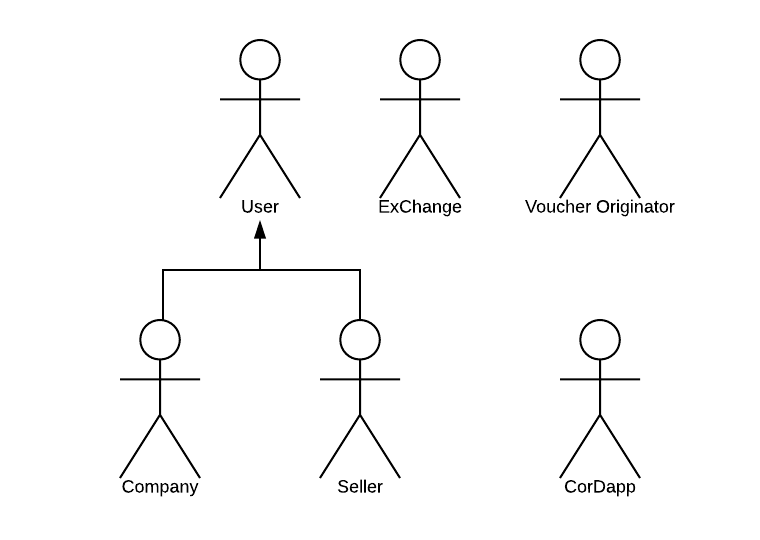
\includegraphics[scale=1]{actors.png}
    \caption{
       Diagram of the actors involved. 
        }
\end{figure}

\subsection{Use Cases}
\begin{enumerate}
    \item \textbf{Generic user use cases}: 
        \begin{itemize}
            \item \textbf{Manage account}: A user can manage their own informations recorded on the application.
            \item \textbf{Adding credits}: A user can add credits, be it fixed value or currency, to their account.
            \item \textbf{Send payment request}: A user can initiate a transaction over the purchase of a good. At the end of the transaction, the value of the good will be added to their account. The user in this case is a seller.
            \item \textbf{Accept payment request}: A user can respond to a transaction over the request of purchase of a good. At the end of the transaction, the value of the good will be detracted from their account. The user in this case is a buyer.
        \end{itemize}
    \item \textbf{Company use cases}: 
        \begin{itemize}
            \item \textbf{Pooling credits}: A company can pool credits from its (willing) employee for a batch order. These orders can be meal orders. The pooling tries to address change leftovers by minimizing it over larger purchases.
            \item \textbf{Redeem a fixed value credit}: Companies with a selling profile can redeem fixed value credits, such as vouchers, from their originators.
            \item \textbf{Send payment request}
            \item \textbf{Accept payment reques}
        \end{itemize}
    \item \textbf{Voucher originator}
        \begin{itemize}
            \item \textbf{Issue credit}: Voucher originators, according to its contracts with companies, issue vouchers to users.
        \end{itemize}
\end{enumerate}

\begin{figure}[h!]
    \centering
    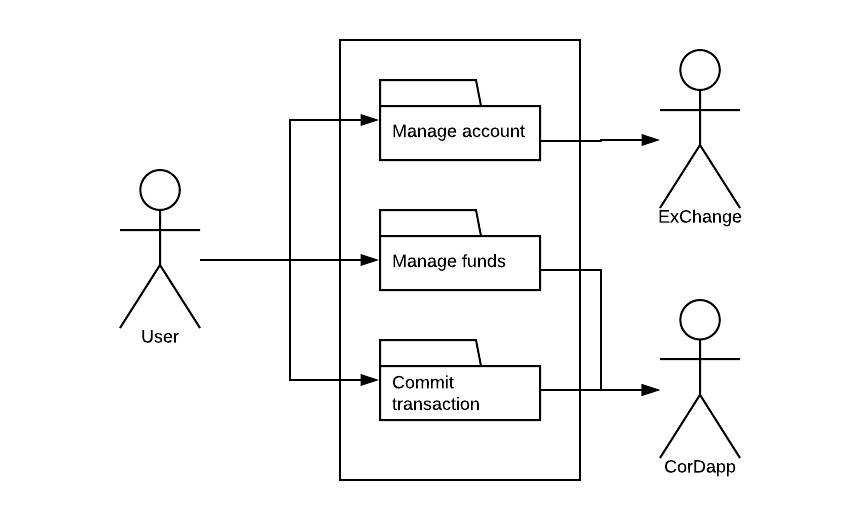
\includegraphics[scale=1]{packages.png}
    \caption{
       Diagram of the use case packages for a generic user.
        }
\end{figure}

\begin{figure}[h!]
    \centering
    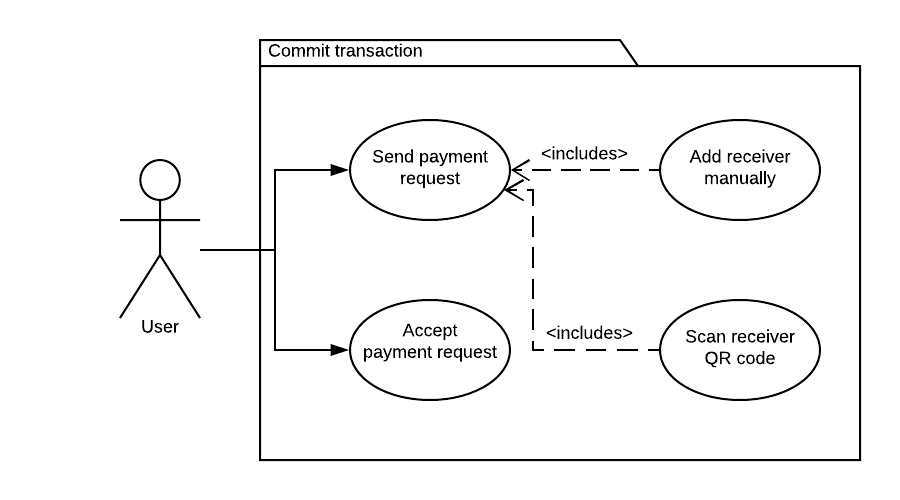
\includegraphics[scale=1]{single-package.png}
    \caption{
       Diagram of a single use case package for a generic user.
        }
\end{figure}

Figures 4.2 and 4.3 show simplified diagrams of a generic user (a buyer or a seller) pertaining use cases, with a focus on the transaction use case package.

The use cases can be clearly partitioned between account management actions, such as editing user information, associated credit card or company, fund management action, such as adding funds and tracking transaction history, and transaction committal actions, such as sending payment requests and accepting payment requests.

We will here on focus on the transactional procedures, as it's the one most closely related to the workings of distributed ledger architecture and Corda itself.

\newpage

\subsection{System architecture}

Before delving into the behavior of the system, it can be useful to consider the architecture of the system.
While we're relatively free to choose how to design the application, or the higher layer "interface" through which the user communicates, we have to take choices about how the application is linked to the distributed ledger underlying architecture provided by Corda. (Note: by high layer interface, it is not meant front-end, as the application can be a built as a complete stand-alone application interfacing the distributed ledger network).
Thus, it is necessary at this point of the process to consider some more technical elements to choose how the system behaves and communicates as a whole.

We will consider the whole system as comprised of two separate subsystems. One is the ExChange application, that acts as an interface for user interaction, and the other is the CorDapp, that is the subsystem that manages the node interactions in the distributed ledger network. 
The CorDapp and its higher level interface do not have to reside in the same enviroment. In this prototype a more coupled solution has been preferred for an easier implementation, so the ExChange application resides in the same enviroment as the CorDapp. 

The ExChange network in its entirety can be considered as the network comprised of users (buyers, sellers, companies, and voucher originators). In addition, the network can present different permissioning services that can be interfaced through the application, such as notaries, oracles or doorman (useful to provide a network map that would work as a map of affiliated shops or premises).
Note that at this point in time Corda still does not provide complete implementation for some of this services (such as the network map), so their design and implementation will be postponed until a further date.

A CorDapp possesses a vault, that contains all the current and historic states that a node is aware of. The vault contains the credits (vouchers, currency) under the form of states, that make up the fund of an user account, and their history - how each state evolved. 

States come in different types. Some states can be transferred through ownership change and some states can be splittable, for example a state describing the ownership of 20 vouchers can be split on necessity in two voucher states (19+1).
A historic state is a state that has been consumed - it evolved from one (or more) state to another.

States evolve through transactions. Each transaction is validated by a smart contract. Smart contracts verify transaction validity, and are a set of rules a transaction has to satisfy to be valid. Different type of transactions are validated by different type of smart contracts.

A flow is the automatization of a transaction - different flows pertain to different transaction types. This architecture expects the creation of a Voucher Payment flow that deals with voucher payments and handling its leftover changes, when existing.

Flows and transaction are regulated with notaries nodes. Notaries guarantee uniqueness consensus and prevent double-spend in the system by running validity controls on the history of states.

\begin{figure}[h!]
    \centering
    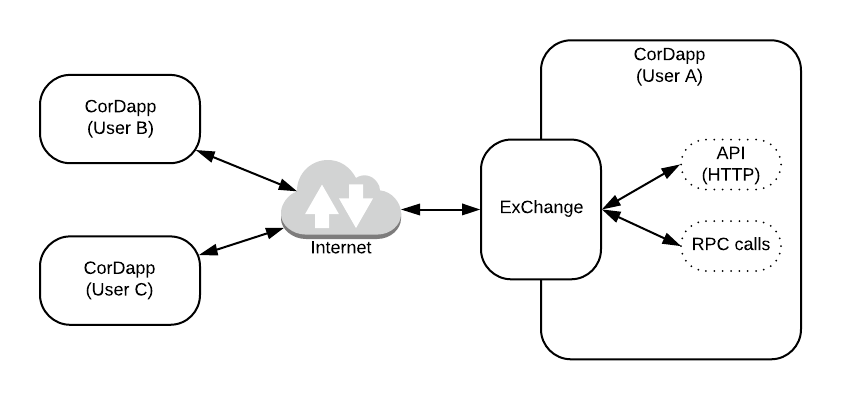
\includegraphics[scale=0.8]{system-architecture.png}
    \caption{
       Simplified architecture of the system.
        }
\end{figure}

\begin{figure}[h!]
    \centering
    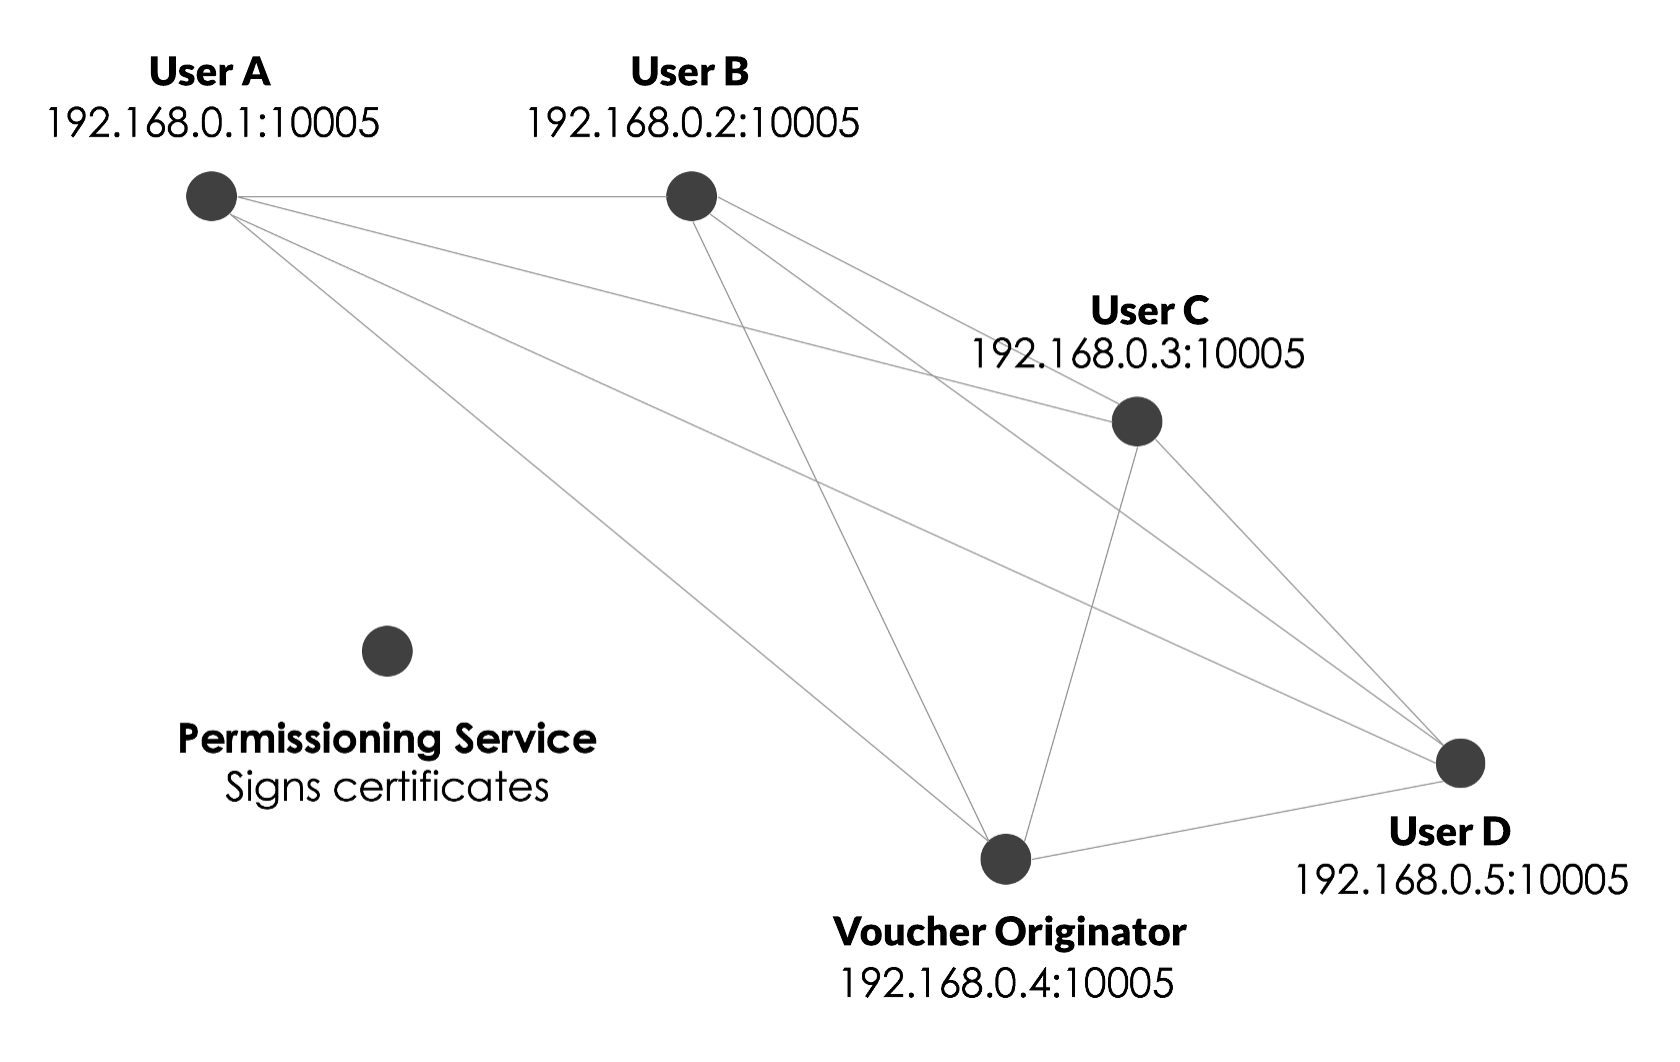
\includegraphics[scale=0.35]{system-network.png}
    \caption{
       Diagram of the ExChange network.
        }
\end{figure}

\newpage

\subsection{System behavior}

Every interaction that involves transactions is managed through the CorDapp. The ExChange application works as a mediator between the requests of the user and the underlying CorDapp. This premise makes it so every action pertaining such use case has to go through two layers: the ExChange app and the underlying CorDapp. 
For the following diagrams we will consider the ExChange application and CorDapp as one single object to underline how the system behaves and communication flows between nodes to commit a transaction.

Figure 4.4 shows the sequence diagram for a would-be purchase using vouchers (it includes also the initial voucher issuance from the originator).
Note that each object in the diagram is a node, and the exchange of messages on a higher level happens through the ExChange application, while the flow is the real transaction that happens in the CorDapp and updates the ledgers of both parties with the transaction.

\begin{figure}[h]
    \centering
    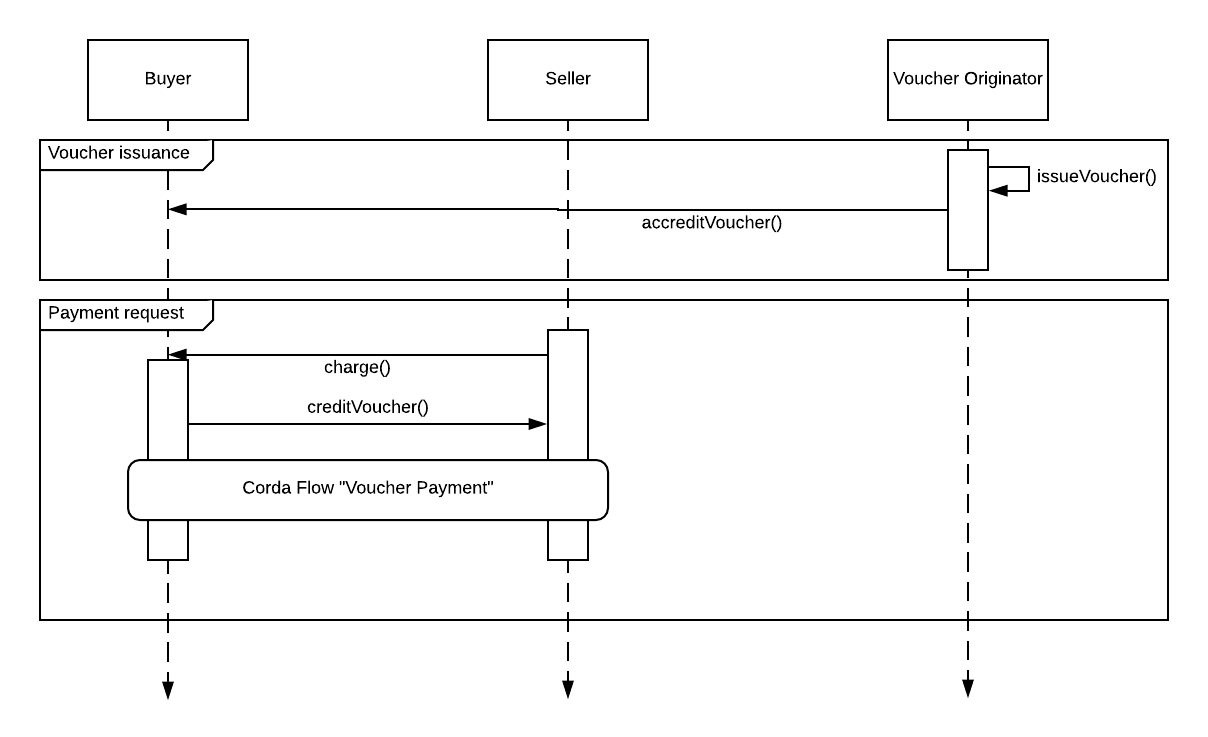
\includegraphics[max size={\textwidth}{\textheight}]{ssd1.png}
    \caption{
       Sequence diagram comprising of voucher issuance and voucher payment.
        }
\end{figure}

\begin{figure}[h]
    \centering
    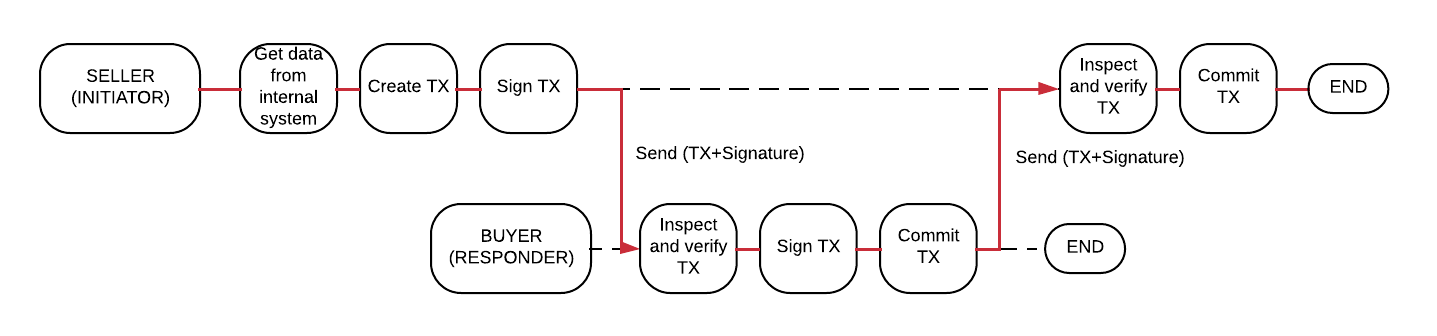
\includegraphics[max size={\textwidth}{\textheight}]{flow.png}
    \caption{
       Diagram of the Voucher Payment flow.
        }
\end{figure}



To understand the transactional process better, we will consider in detail how a voucher payment works and how the states in the ledger change.

\subsection{Voucher payments}

Two solutions have been elaborated to solve the issue of voucher payments and leftover change.

Both solutions provide advantages in terms of automatization of the voucher payment process and change processing - not considering the advantages and securities offered by the DLT itself.

The first solution, in case of mismatch between payment request and voucher face value presupposes the creation of IOUs in the vault of the seller. IOUs in this case are discount states representing the leftover change from the voucher. 

\begin{figure}[h!]
    \centering
    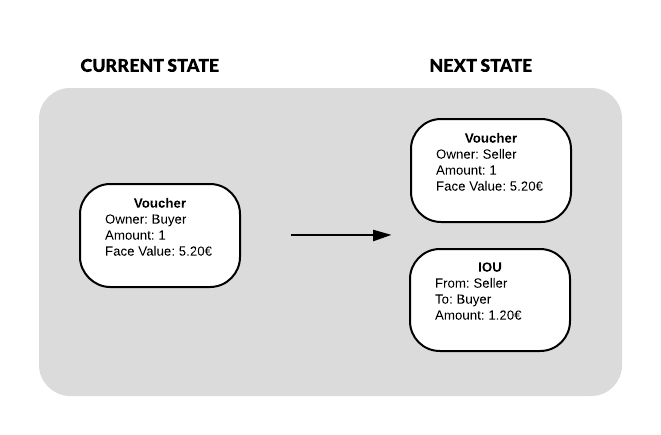
\includegraphics[max size={\textwidth}{\textheight}]{states-ex.png}
    \caption{
       Input and output states by the "Voucher Payment" flow in the distributed ledger viewed by the buyer and the seller.
        }
\end{figure}

Figure 4.8 represents the distributed ledger contents between the buyer and seller nodes, before and after a payment transaction of 4€ with a voucher with a face value of 5.20€ according to the first solution. 

The buyer will retain the change for future payments and purchases from the same seller.
How the states are consumed in the transaction depends on the final implementation of the flow. The Voucher Payment flow can be setup so it consumes the most optimal combination of states, giving priority to IOU states - if existing in the seller vault - and then voucher states.

This solution presents no added risks from either parties compared to a normal transaction, and automatizes the handling of voucher's leftover change.
It is somewhat more rigid than preferred, as the change's future usage is limited to the seller where it was generated.

The second solution enables transferrable change. After a voucher payment, a change state is generated in the buyer's vault, corrisponding to the change left over by the voucher.
It is here necessary to introduce a second type of voucher state, called "Redeemable Voucher". Redeemable Voucher states represent list of vouchers detained by a seller.
A seller can effectively redeem only the redeemable amount of voucher they own. 

Figure 4.9 represents the distributed ledger before and after a payment transaction of 4€ with a voucher with a face value of 5.20€ according to the second solution. If a buyer uses a 5.20€ voucher to pay for a 4€ good, he is given a 1.20€ change state, which they can use without any limitation to the seller. 
The seller, on other hand, cannot redeem the 5.20€ voucher in its entirety, as he only obtained 4€ worth of it. 

This arises the issue of how to deal with voucher fragmentation, as this leaves the seller open to eventual malicious "voucher exchange" attacks - that is an attack where a buyer might use a voucher for a small purchase, for example of 0.10€, to cash in the change and leave to the seller the burden of accumulating the 5.10€ of difference needed to redeem the voucher. 

Voucher fragmentation can be dealt easily as Sellers can use their own funds in their accounts to issue change free from vouchers - the change can be any other kind of transferrable credit accepted by the platform, for example, currency.

\begin{figure}[h!]
    \centering
    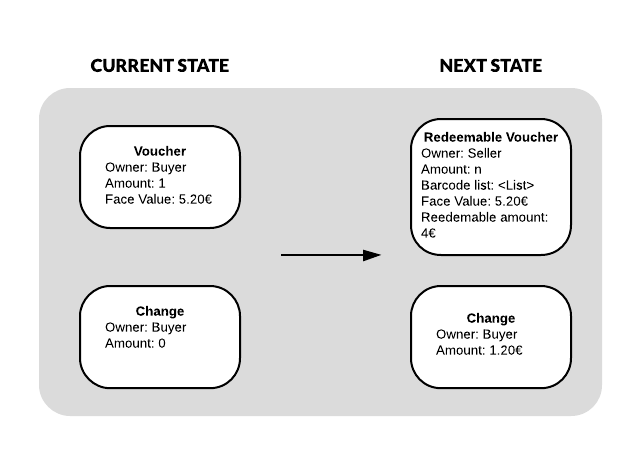
\includegraphics[max size={\textwidth}{\textheight}]{states-ex2.png}
    \caption{
       Input and output states by the "Voucher Payment" flow in the distributed ledger viewed by the buyer and the seller.
        }
\end{figure}

A note has to be said in regards of the second solution here shown. The entire implementation of such solution is only a thought experiment in regards to how to deal with voucher leftover changes, as the conversion of change leftover into an effective digital credit to be used in a transactional platform isn't regulated.


\section{Implementation}

\begin{figure}[h!]
    \centering
    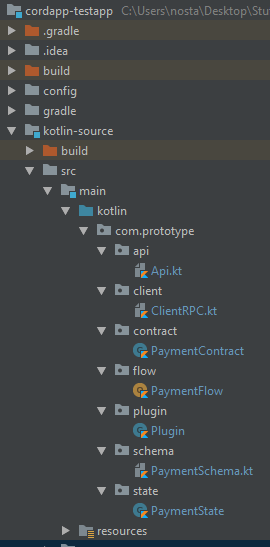
\includegraphics[scale=0.6]{project-structure.png}
    \caption{
       Structure of the Corda implementation
        }
\end{figure}

A test application implementing the basic communication between nodes and exchange of a "Payment" state has been implemented in Kotlin using the IntelliJ IDEA environment. The test application regards only the CorDapp subsystem, and allows a seller node and a buyer node to agree on a payment, if it follows the following contract rules: 

\begin{itemize}
    \item The payment's value is strictly positive
    \item A node is not trying to pay itself
\end{itemize}

The CorDapp can be deployed as three nodes, Buyer, Seller, and Notary.
The Corda Kotlin template has been used for the development of this test application.

\newpage

\subsection{State}

The first class to define is the state class, representing the shared facts on the ledger. The class is immutable, meaning that the values of one instance of the class cannot be modified. Instead, consumed states become historic, and a new state with new values is put into its sequence.

\begin{figure}[h]
    \centering
    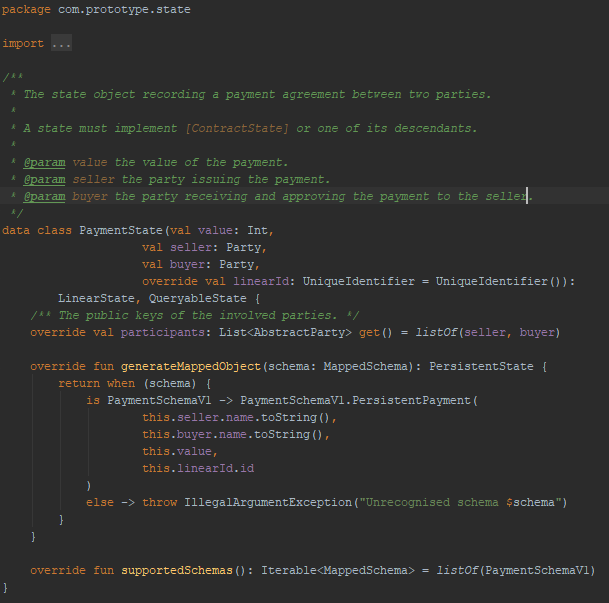
\includegraphics[scale=0.8]{project-state.png}
    \caption{
       Payment state class
        }
\end{figure}

\newpage

\subsection{Contract}

The contract class is used to define how an associated state evolves over time. In Corda, contracts also are able to impose what kind of transactions are to be allowed, so when input and output states do not satisfy a contracts rules, the transaction is considered invalid.

\begin{figure}[h]
    \centering
    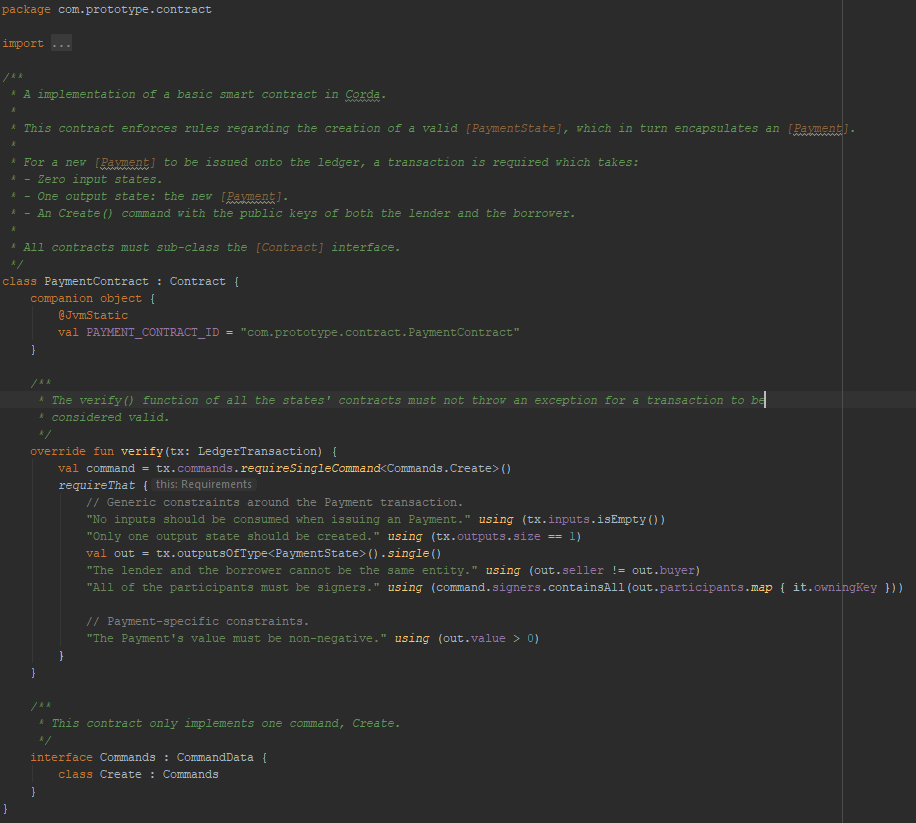
\includegraphics[max size={\textwidth}{\textheight}]{project-contract.png}
    \caption{
       Payment contract class
        }
\end{figure}


\newpage

\subsection{Flow}

The flow class allows to define the steps needed for a Corda node to perform an update on the ledger. In other words, flows allows nodes to issue new PaymentStates to the ledger. Every flow has two sides, the Initiator side, which will initiate the request to update the ledger, and the Acceptor side, which will respond to said request.

\begin{figure}[h]
    \centering
    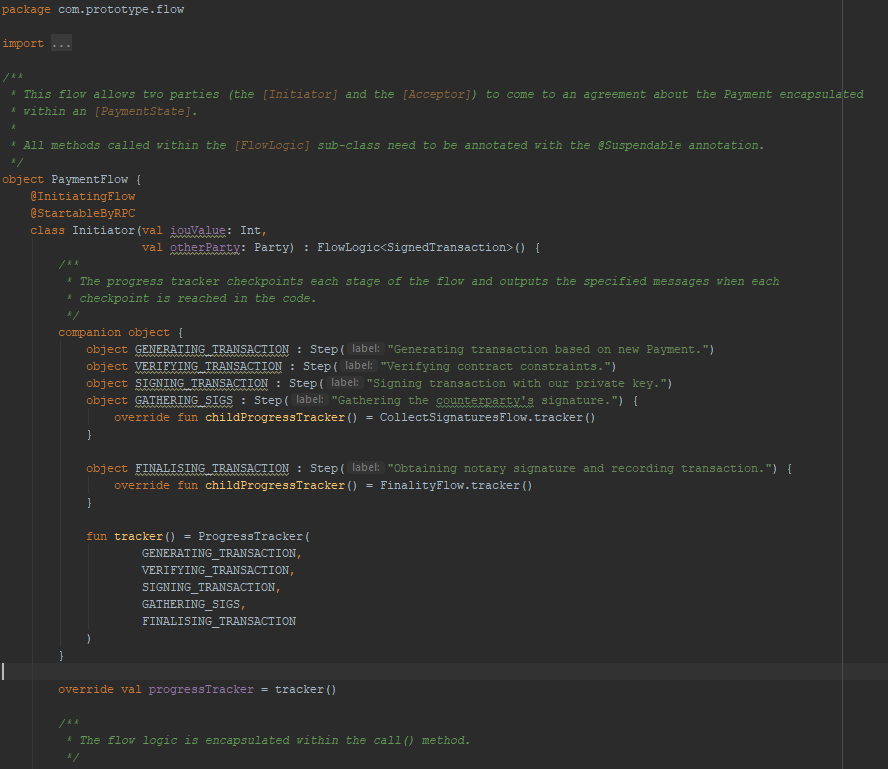
\includegraphics[max size={\textwidth}{\textheight}]{project-flow1.png}
    \caption{
        Payment flow class
         }
\end{figure}
\begin{figure}[h]
    \centering
    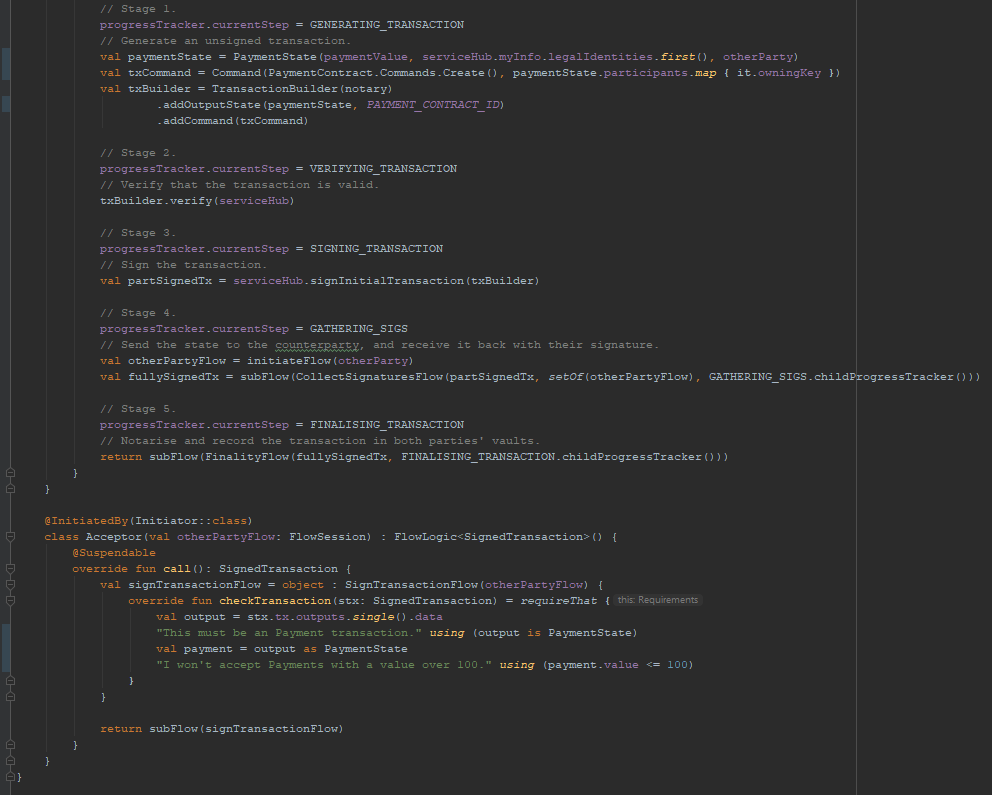
\includegraphics[max size={\textwidth}{\textheight}]{project-flow2.png}
    \caption{
        Payment flow class
         }
\end{figure}

\newpage

\subsection{Interaction}
The front-end and API haven't been fully implemented (ExChange application), as they are outside the scope of this project. A command line interface has been implemented to interact with the network via command line. It is possible to run the client on the terminal window, with the commands:
\begin{verbatim}
  cd project
  ./gradlew clean deployNodes
  ./build/nodes/runnodes 
\end{verbatim}

\begin{figure}[h]
    \centering
    
\includegraphics[]{logo_unimib.pdf}
    \caption{
        deployNodes task in the build.gradle file
         }
\end{figure}

With that it's possible to verify that the nodes and implemented classes are running correctly.